\section{Identyfikacja}

W ramach identyfikacji obiektu wyznaczono charakterystyki statyczne oraz zbadano odpowiedzi zbiorników na wymuszenia skokowe dopływów - $F_1$ oraz $F_D$. Ponadto dokonano porównania modelu liniowego i nieliniowego.

\subsection{Charakterystyka statyczna}
Charakterystyka statyczna obiektu to zależność między sygnałem wejściowym a odpowiadającym mu sygnałem wyjściowym w stanie ustalonym, czyli po zaniku procesów przejściowych. Opisuje ona zachowanie systemu w warunkach statycznych, bez uwzględniania dynamiki i opóźnień. W identyfikacji obiektu pozwala określić jego nieliniowości oraz przewidzieć, jak wyjście reaguje na różne wartości wejścia. W przedstawianej pracy poświęcono jej bardzo dużo uwagi, ze względu na istotną rolę, jaką odgrywa we wspomnianych modelach Hammersteina i Wienera. Dzięki niej można uprościć identyfikację parametrów, analizując najpierw charakterystykę statyczną, a dopiero potem właściwości dynamiczne systemu. Korzystając z modelu fizycznego, z równania \ref{model_fiz} wyznaczono:

\begin{equation}
\frac{dV_1}{dt} = 0 \quad \wedge \quad \frac{dV_2}{dt} = 0
\end{equation}

\noindent wobec tego:
\begin{equation}
\begin{cases}
0 &= F_1 + F_D - \alpha_1 \sqrt{h_1} \\[10pt]
0 &= \alpha_1 \sqrt{h_1} - \alpha_2 \sqrt{h_2}
\end{cases}
\end{equation}

\noindent Po przekształceniach otrzymano wzór opisujący charakterystykę statyczną:
\begin{equation}
h_2 = \left( \frac{F_1 + F_D}{\alpha_2} \right)^2
\end{equation}

\noindent Wykres odpowiadający wyprowadzonemu wzorowi, w zależności od danej zmiennej - sterowanie lub zakłócenie - prezentuje się następująco:

\begin{figure}[h!]
\centering
\subfloat[$h_2(F_1)$]{
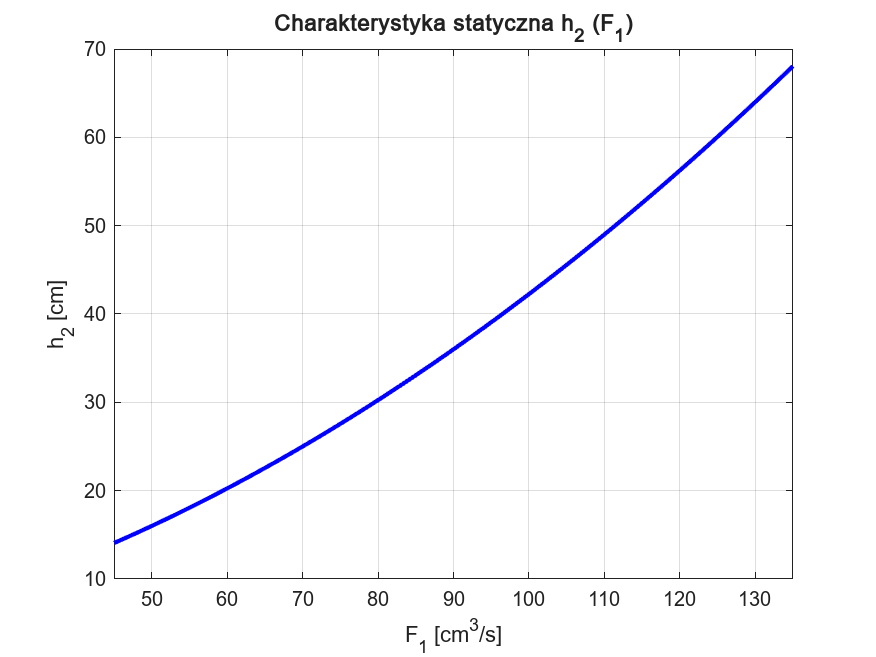
\includegraphics[width=0.475\textwidth]{pictures/static_characteristic_F1}}
\quad
\subfloat[$h_2(F_D)$]{
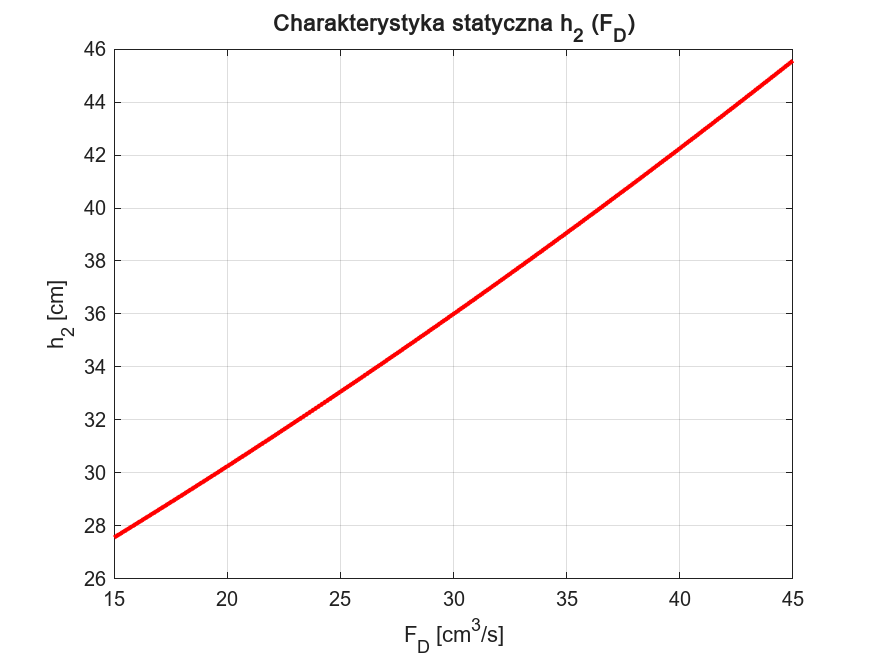
\includegraphics[width=0.475\textwidth]{pictures/static_characteristic_FD}}
\caption{Charakterystyka statyczna.}
\end{figure}

\newpage

\begin{figure}[h!]
\centering
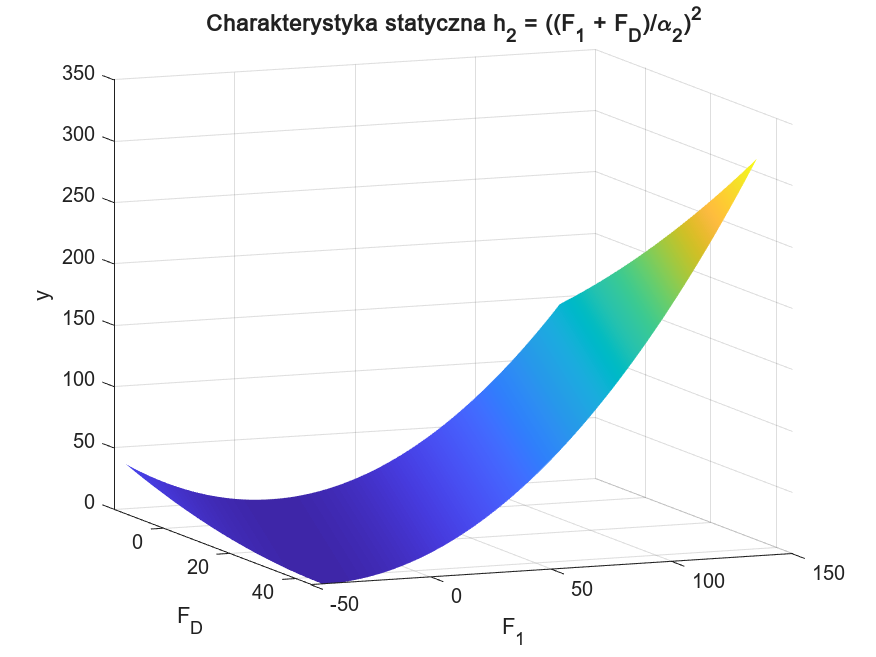
\includegraphics[width=\textwidth]{pictures/static_characteristic_3D}
\caption{Trójwymiarowa charakterystyka statyczna.}
\end{figure}

\noindent Otrzymano spodziewane przebiegi, mianowicie w obu przypadkach wykresy przedstawiają parabole. Podczas wyznaczania charakterystyk założono przedziały zmienności zmiennej sterującej oraz zakłócenia:
\begin{itemize}
\item[•] $F_1 \in [45, 135]$, co odpowiada przyrostowi $\Delta F_1 \in [-45, 45]$
\item[•] $F_D \in [15, 45]$, co odpowiada przyrostowi $\Delta F_D \in [-15, 15]$
\end{itemize}

\newpage

\subsection{Porównanie modelu liniowego i nieliniowego}

Wykresy charakterystyk statycznych uzupełniono serią wymuszeń skokowych, które prezentowały się następująco:

\begin{figure}[h!]
\centering
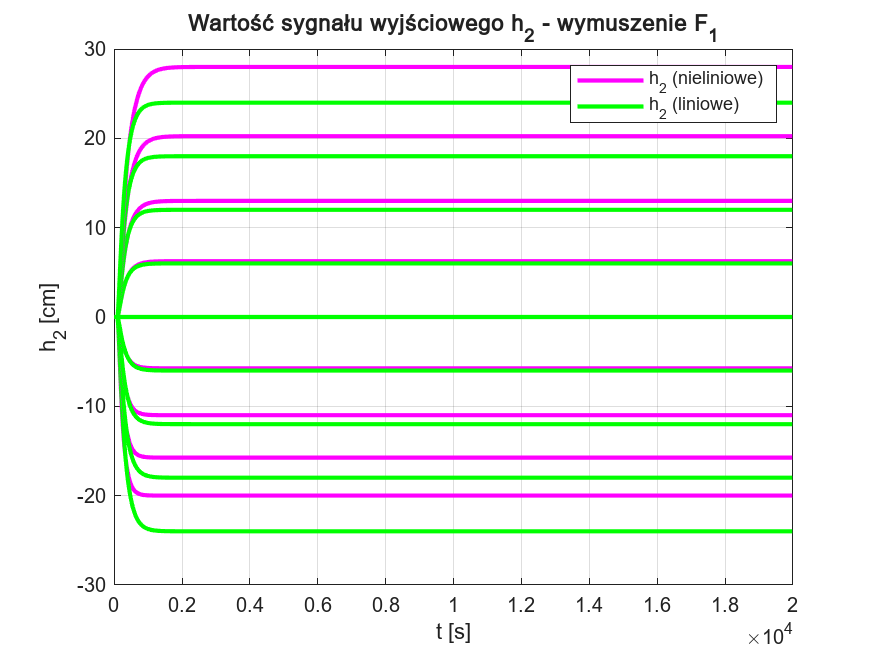
\includegraphics[width=0.8\textwidth]{pictures/wymuszenie_F1}
\caption{Porównanie odpowiedzi obiektu nieliniowego i zlinearyzowanego w punkcie pracy na wymuszenia skokowe sygnału $F_1$.}
\end{figure}

Otrzymano spodziewane przebiegi, mianowicie, blisko punktu linearyzacji model liniowy odzwierciedla rzeczywiste zachowanie układu, natomiast wraz z oddalaniem się od punktu pracy ta dokładność maleje. Utratę tę dokładności przedstawiono w Tab. \ref{errors_F1}, obliczając dla każdej pary odpowiedzi liniowej i nieliniowej, błąd średniokwadratowy, tj.

\begin{equation}
E = \frac{1}{kk} \sum_{k=1}^{kk} (y(k) - y_L(k))^2
\end{equation}

\begin{table}[h!]
\centering
\renewcommand{\arraystretch}{1.2} % Zwiększa wysokość wierszy
\begin{tabular}{|>{\centering\arraybackslash}m{3cm}|>{\centering\arraybackslash}m{3cm}|}
\hline
Wymuszenie & Błąd \\ \hline
$F_{10} - 40$ & $\num{15.427}$ \\ \hline
$F_{10} - 30$ & $\num{4.875}$ \\ \hline
$F_{10} - 20$ & $\num{0.962}$ \\ \hline
$F_{10} - 10$ & $\num{0.060}$ \\ \hline
$F_{10}$ & $\num{0.000}$ \\ \hline
$F_{10} + 10$ & $\num{0.060}$ \\ \hline
$F_{10} + 20$ & $\num{0.956}$ \\ \hline
$F_{10} + 30$ & $\num{4.830}$ \\ \hline
$F_{10} + 40$ & $\num{15.235}$ \\ \hline
\end{tabular}
\caption{Wartość błędu średnio kwadratowego w zależności od wielkości wymuszenia $F_1$.}
\label{errors_F1}
\end{table}

\newpage

Charakter odpowiedzi obiektu na wymuszenia $F_D$ wyglądał analogicznie do, wcześniej zaprezentowanych, wymuszeń $F_1$.

\begin{figure}[h!]
\centering
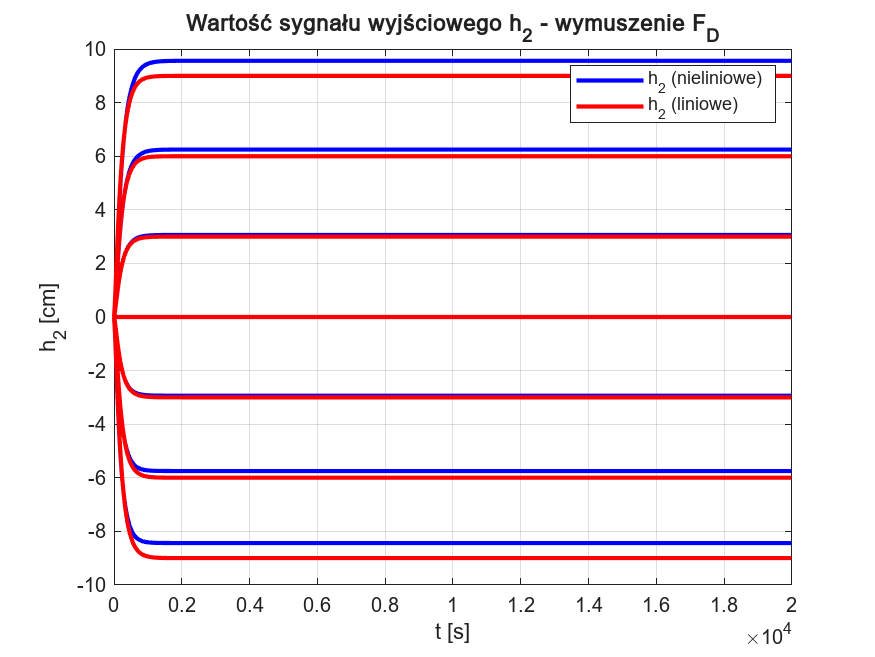
\includegraphics[width=0.8\textwidth]{pictures/wymuszenie_FD}
\caption{Porównanie odpowiedzi obiektu nieliniowego i zlinearyzowanego w punkcie pracy na wymuszenia skokowe sygnału $F_D$.}
\end{figure}

\begin{table}[h!]
\centering
\renewcommand{\arraystretch}{1.2} % Zwiększa wysokość wierszy
\begin{tabular}{|>{\centering\arraybackslash}m{3cm}|>{\centering\arraybackslash}m{3cm}|}
\hline
Wymuszenie & Błąd \\ \hline
$F_{10} - 15$ & $\num{0.306}$ \\ \hline
$F_{10} - 10$ & $\num{0.060}$ \\ \hline
$F_{10} - 5$ & $\num{0.004}$ \\ \hline
$F_{10}$ & $\num{0.000}$ \\ \hline
$F_{10} + 5$ & $\num{0.004}$ \\ \hline
$F_{10} + 10$ & $\num{0.060}$ \\ \hline
$F_{10} + 15$ & $\num{0.304}$ \\ \hline
\end{tabular}
\caption{Wartość błędu średnio kwadratowego w zależności od wielkości wymuszenia $F_D$.}
\end{table}

Z racji na założony mniejszy przedział zmienności sygnału zakłócającego, różnice między modelem liniowym, a nieliniowym nie były tak duże jak w przypadku sygnału sterującego.